% Classe do documento e parâmetros gerais.
\documentclass[a4paper,openright,twoside,11pt]{report}

% Packages utilizadas e respetivos parâmetros.
\usepackage[utf8]{inputenc}
\usepackage[portuguese]{babel}
\addto{\captionsportuguese}{\renewcommand{\bibname}{Refer\^{e}ncias}}
\addto{\captionsportuguese}{\renewcommand{\contentsname}{\'{I}ndice de Conte\'{u}dos}}
\addto{\captionsportuguese}{\renewcommand{\appendixname}{Ap\^{e}ndice}}

\usepackage{lipsum} % gerador de texto
\usepackage{graphicx}
\usepackage{url}
\usepackage[Algoritmo]{algorithm}
\usepackage{algorithmicx}
\usepackage{algpseudocode}
\usepackage{grffile}
\usepackage{caption}
\usepackage{xcolor}

%\usepackage{hyperref}
\usepackage[colorlinks]{hyperref}

\hypersetup{
    colorlinks = true,
    linkbordercolor = {white},
    linkcolor = {blue}, %links dos capitulos e imagens
    citecolor = {blue} %referencias
}

%\usepackage[outdir=./diagramas]{epstopdf}
%\usepackage[utf8]{inputenc}

\renewcommand{\algorithmicrequire}{\textbf{Dados: }}
\renewcommand{\algorithmicensure}{\textbf{Resultado: }}


% Definições das dimensões das páginas
\setlength{\textheight}{24.00cm}
\setlength{\textwidth}{15.50cm}
\setlength{\topmargin}{0.35cm}
\setlength{\headheight}{0cm}
\setlength{\headsep}{0cm}
\setlength{\oddsidemargin}{0.25cm}
\setlength{\evensidemargin}{0.25cm}

%\renewcommand{\baselinestretch}{1}

% Página inicial (capa)
\title{
   \vspace{-50mm}
   \begin{minipage}[l]{\textwidth}
      \hspace{-20mm}\resizebox{75mm}{!}{
\includegraphics{./diagramas/logoISEL.png}}\\
   \end{minipage}\\[10mm]
   {\bf Sistema de Leitura de Contadores de Consumos de Água por Dispositivo Móvel -\textit{Water Watcher} }
	\begin{center}
      	\resizebox{50mm}{!}{
\includegraphics{./diagramas/logoww.png}}\\
      \end{center}
}

% Nome dos autores (um por linha)
\author{
\begin{tabular}{ll}
	Lucas Silva, n.º 44862, e-mail: a44862@alunos.isel.pt\\
\end{tabular}}

\date{
\begin{tabular}{ll}
{Orientadores:} & Carlos Gonçalves, e-mail: carlos.goncalves@isel.pt\\
                 & Luís Osório, e-mail: lo@isel.ipl.pt\\
\end{tabular}\\[10mm]
% Deixar o indicador respetivo em função da versão do relatório.
Relatório do projeto realizado no âmbito de Projecto e Seminário\\
Licenciatura em Engenharia Informática e de Computadores\\[20mm]
Maio de 2021}

%Gloss-------------------------------------------------------------------------------------------------------------------------------------------------------------------------------------------------------------------------------------------------------------------------------------
%\makeglossaries

%\label{smas}
%\newacronym{smas}{SMAS}{Serviços Municipalizados de Água e Saneamento}
%\newacronym{pwa}{PWA}{Progressive Web Applications}

%------------------------------------------------------------------------------------------------------------------------------------------------------------------------------------------------------------------------------------------------------------------------------------




\begin{document}
\pagenumbering{roman}
\thispagestyle{empty}
\maketitle

\baselineskip 18pt % line spacing: 12pt for single, 18pt for 1 1/2, and 24pt for double spacing

\newpage
\thispagestyle{empty}
% Fim da contracapa

% Página com identificação completa (número e nome) e assinaturas do(s) estudante(s) e do(s) orientador(es)
\cleardoublepage
\setcounter{page}{1}
\begin{center}
\textsc{\LARGE Instituto Superior de Engenharia de Lisboa}\\[50mm]

{\large \bf   Sistema de Leitura de Contadores de Consumos de Água por Dispositivo Móvel - \textit{Water Watcher}}\\[20mm]

\begin{tabular}{rl}
  44862  & Lucas Neves da Silva\\[10mm]
           & \rule{75mm}{0.5pt}\\[5mm]
\end{tabular}\\[10mm]

\begin{tabular}{rl}
  Orientadores: & Carlos Gonçalves\\[10mm]
                & \rule{75mm}{0.5pt}\\[5mm]
                & Luís Osório\\[10mm]
                & \rule{75mm}{0.5pt}\\
\end{tabular}\\[10mm]

Relatório do projeto realizado no âmbito de Projecto e Seminário\\
Licenciatura em Engenharia Informática e de Computadores\\[20mm]
Maio de 2021\\
\end{center}

% Página de resumo em Português
\cleardoublepage
\chapter*{Resumo}
O processo de envio de leituras de consumo de água é um processo tecnologicamente desatualizado, na medida que o cliente paga, por norma, um valor baseado num consumo estimado, pelo que é frequente existirem erros nas estimativas, cuja resolução é algo morosa e burocrática.\\
Este projeto pretende colmatar estas situações, propondo a implementação de um sistema informático que permite ao cliente indicar facilmente à empresa o valor que realmente consumiu, não sendo assim necessários acertos de pagamento e permitindo ao cliente e à empresa ter um controlo do valor real de água consumida.\\
O sistema também apresentará ao utilizador estatísticas e infromações relativas a este serviço, bem como informá-lo-á de situações relacionadas com o pagamento ou outros eventos relacionados.
\vspace{1.5cm}

{\bf Palavras-chave:} Leituras de Contadores de Água; Sistema Informático; Progressive Web Apps.

\cleardoublepage %GLOSS ------------------------------------------------------------------------
\chapter*{Glossário de Termos}

\begin{tabular}[l]{l  p{11cm}} 

Interface de Utilizador: & Apresentação gráfica dos dados e funcionalidades de um elemento que possibilita interação.\\ 

PWA:  & Progressive Web Applications\\

SMAS: & Serviços Municipalizados de Água e Saneamento\\

\end{tabular}
\label{tab:req_utilizador}

%% Página de agradecimentos
%\cleardoublepage
%\chapter*{Agradecimentos}
%Texto dos agradecimentos. É opcional.\\

% Geração do índice de conteúdos
\cleardoublepage
\tableofcontents \cleardoublepage


% Geração do índice de figuras e de tabelas
%\listoffigures \cleardoublepage
%\listoftables \cleardoublepage

% Reiniciar a numeração de páginas
\setcounter{page}{1}
\pagenumbering{arabic}

% Capitulo 1
%
% Capítulo 1
%
\chapter{Introdução} \label{cap:intro}

A vasta maioria das casas, lojas e escritórios recorrem a serviços de abastecimento de água. O custo deste serviço é calculado, normalmente, através de uma estimativa da quantidade de água gasta (por norma mensalmente) e, periodicamente, um funcionário da empresa que fornece o serviço tem de se deslocar à localização do contador para que seja verificado o consumo real de água para o acerto do pagamento. 
O crescimento tecnológico contemporâneo facilitou e incentivou o acesso de grande parte da população aos vários equipamentos e plataformas tecnológicas que nos permitem efetuar diversas tarefas que outrora necessitariam de outra burocracia ou até serviço presencial. A entrega da leitura da contagem da água é algo que pode ser modernizado e automatizado, porém reconhecemos que soluções que envolvam, por exemplo, a substituição dos equipamentos contadores, possam acarretar um custo logístico e financeiro não justificável para a empresa. 
Neste projeto, propomos uma solução que permite modernizar o processo de entrega de leituras de água apenas envolvendo a implementação de um sistema informático que permite aos clientes enviar fotografias dos seus contadores que depois o sistema processará para obter o valor da contagem.


%
% Secção 1.1
%
\section{Objetivo} \label{sec11}

De forma a não ser necessário fazer acertos de pagamentos e permitir que o cliente pague realmente o valor que consumiu, ao invés do consumo estimado, este projeto tem como propósito o desenvolvimento de um sistema informático composto por, de entre outros elementos, um elemento que o cliente utiliza para comunicar ao fornecedor o seu consumo de água. Este poderá também ser utilizado para indicar estatísticas de consumo e notficar o cliente de informações pertinentes relativas a este serviço. Para além deste elemento, também vai ser realizado um servidor cuja função principal é comunicar com o elemento dos utilizadores e interagir com o local onde estão guardadas as informações dos clientes.

\section{Organização do Documento} \label{sec12}
O restante relatório encontra-se organizado em quatro capítulos. No capítulo \ref{cap:trabrelacionado} vamos avaliar e debater soluções já existentes no mercado cuja função se aproxima da deste projeto, bem como os vários equipamentos e conceitos utilizados na área cujo projeto se insere. No capítulo\ref{cap:analise} estudaremos os vários problemas do projeto, detalhando os vários requisitos que o sistema terá de cumprir para satisfazer o seu propósito. 
%O capítulo \ref{cap:trabrelacionado} será onde vamos comparar e explicar as várias estratégias de abordagem às soluções apresentadas.
% Por fim, o capítulo 5 (Aspetos de Implementação) será onde vamos analisar diretamente o código fonte da solução e explicar os diversos detalhes e escolhas efetuadas durante a escrita do código.

% Capitulo 2
%
% Capítulo 2
%
\chapter{Trabalho Relacionado} \label{cap:trabrelacionado}
Neste capítulo vamos abordar sistemas relacionados com o nosso trabalho e alguns sistemas semelhantes ao que vamos desenvolver. Vamos também debater sobre algumas tecnologias e plataformas que vamos utilizar no desenvolvimento do projeto.\\
A elaboração deste projeto envolve vários componentes externos, pelo que será importante analisar os vários componentes com os quais vamos interagir.\\
Na secção \ref{sec:cont} vamos analisar os contadores de água com os quais o nosso sistema vai interagir. Nas secções \ref{sec:appsmas} e \ref{sec:telemetria} vamos abordar algumas soluções já existentes no mercado com funções semelhantes à do sistema que vamos desenvolver.Na secção \ref{sec:pwa} vamos apresentar o tipo de sistema que vamos desenvolver e na secção \ref{sec:outsystems} a ferramenta que vamos utilizar para o desenvolver.


\section{Contadores de Água} \label{sec:cont}
Para a realização deste projeto é importante analisar os dispositivos contadores de água, dado que o nosso sistema vai interagir com eles, nomeadamente, obtendo a sua medição.
Existem vários tipos de contadores de água, diferindo na aparência, no contexto que devem ser utilizados (residencial, comercial, industrial) ou na forma como registam a quantidade de água que passa por eles. Para este projeto, nós vamos interagir apenas com o dispositivo indicador, que é o local do contador que indica a leitura de água e o seu número de série.
A figura \ref{fig:contador} contém uma imagem de um contador, onde podemos observar no retângulo 1 ( a verde) a medição do contador e no retângulo 2 (a azul) o ano e número de série do contador.

\begin{figure}[h!]
\begin{center}
\resizebox{80mm}{!}{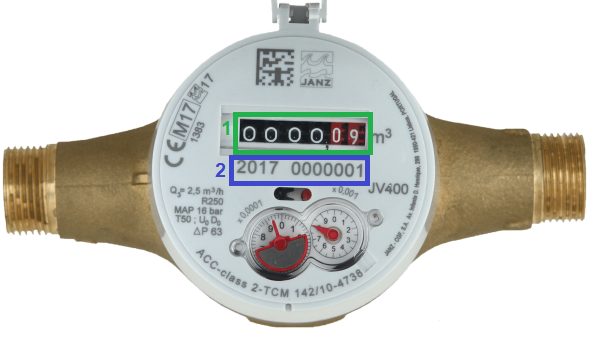
\includegraphics{diagramas/contador.png}}
\caption{Dispositivo indicador do contador de água.}
\label{fig:contador}
\end{center}
\end{figure}


Existem sistemas com funções e finalidades próximas ou até iguais ao sistema que vamos conceber. Deveremos analisar as várias funções destes sistemas, porém também as suas falhas e funcionalidades que deveriam ter sido implementadas, para que no nosso sistema possamos colmatar essas situações e oferecer uma solução mais competente e vantajosa.

\section{Aplicação para Dispositivo Móvel} \label{sec:appsmas}
Os Serviços Municipalizados de Água e Saneamento de Almada e de Sintra já possuem, respetivamente, aplicações para \textit{smartphone} \cite{smas:almada} e websites \cite{smas:sintra} para as diferentes zonas em que operam. Estas plataformas permitem a gestão do contrato, consulta de contas, faturas e consumos, ativação de pagamento por débito direto, alteração de dados pessoais e a comunicação de leituras.

\section{Sistemas de Telemetria} \label{sec:telemetria}
Existem, aplicados a esta área, sistemas de telemetria, ou seja, sistemas que efetuam a medição e comunicação das leituras. Alguns destes sistemas vêm incorporados no aparelho contador, existindo também outros que são um dispositivo separado \cite{janz:impji}. Porém, neste último caso, o contador de água tem de ser construído com características próprias que lhe permitam comunicar com estes dispositivos.

\section{Progressive Web Apps} \label{sec:pwa}
Progresive Web Apps (PWA) ou aplicações web progressivas são aplicações que podem funcionar em qualquer dispositivo que possua um web browser, sendo a principal característica que as define ser a junção das vantagens das aplicações web normais e das aplicações nativas, específicas para plataformas. \\
As aplicações web são aplicações que funcionam em qualquer dispositivo que suporte um web browser, como computadores e smartphones. Isto permite-nos ter uma base de código comum que funciona em vários dispositivos, ao contrário do que acontece com as aplicações nativas, o que resulta em construir e suportar menos código. \\
Porém, as PWA permitem-nos, tal como as aplicações nativas e ao contrário das restantes aplicações web, utilizar funções específicas do dispositivo, como aceder à localização, interagir com dados do dispositivo ou utilizar notificações. 

\section{Outsystems Service Studio} \label{sec:outsystems}
Outsystems Service Studio é uma ferramenta que nos permite desenvolver PWAs. Esta ferramenta permite-nos desenvolver as várias componentes do sistema como a lógica do sistema, a sua componente visual de interação com o utilizador e o seu modelo de dados, o que é vantajoso, na medida em que apenas é necessário utilizar uma plataforma para a elaboração do sistema. \\
É considerada uma plataforma ‘low-code’, dado que a plataforma gera automaticamente algum código que podemos utilizar no nosso projeto, o que ajuda no desenvolvimento e manutenção do projeto.



% Capitulo 3
\chapter{Análise do Problema} \label{cap:analise}

Tal como apresentado anteriormente, este projeto consiste na realização do sistema informático que designamos por Water Watcher, constituído por três partes: a interface para os utilizadores, o elemento servidor e o elemento que armazena os dados. Estes irão interagir com o sistema informático que a empresa de sistema de fornecimento de água já possui e utiliza.\\
A figura \ref{fig:modelo} representa o sistema e os seus componentes. O servidor e a interface do utilizador são componentes intrínsecos do sistema, pelo que o sistema não existiria sem eles, enquanto que o sistema de gestão de base de dados será um componente do sistema porém independente. O sistema de gestão de consumos é um outro sistema com o qual o nosso vai comunicar, sendo este sistema o sistema que a empresa fornecedora de água já utiliza para gerir os dados relativos ao seu serviço.

\vspace{1cm} %espaço

\begin{figure}[ht!]
\centering
\resizebox{150mm}{!}{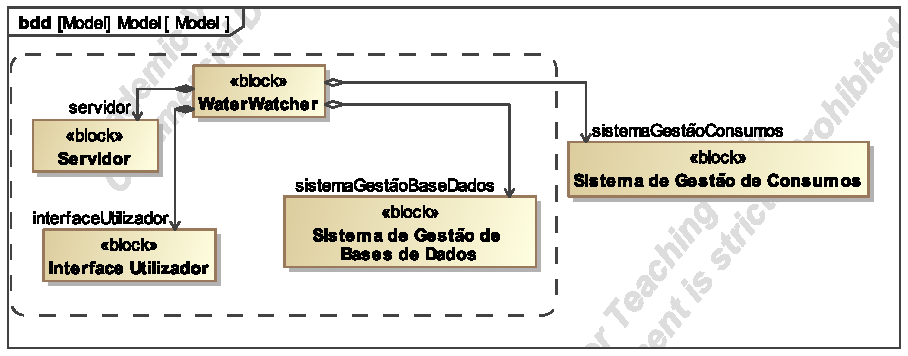
\includegraphics{diagramas/svg/bdd__Model.pdf}}
\caption{Arquitetura do sistema.}
\label{fig:modelo}
\end{figure}

A interface para os utilizadores terá como função principal a “leitura” do contador, ou seja, através da câmara do dispositivo, é capturada uma imagem da contagem medida pelo aparelho contador de consumo de água. Este elemento terá garantias de robustez em cenários de utilização real, isto é, deverá saber lidar de forma correta com situações anómalas como o mau estado dos contadores ou leituras erradas por erro do sistema ou do cliente.\\
Leituras erradas deverão, de forma geral, ser substituídas pela estimativa já calculada pela empresa, ou por uma nova estimativa calculada por este sistema informático.\\
Este componente poderá também apresentar informações relativas ao consumo de água como estatísticas de consumo em intervalos de tempo definidos, aviso de gastos menores/maiores que o esperado e outras possíveis informações pertinentes ao cliente sobre este serviço.\\
Outro elemento deste sistema informático será um servidor, cuja função é, resumidamente, interpretar os caracteres das imagens captadas pelos utilizadores e receber os pedidos de informação das interfaces dos utilizadores, comunicá-los ao elemento que armazena os dados e encaminhar a devida resposta de novo à interface dos utilizadores. Também será o servidor o responsável por assegurar a integridade das comunicações, como verificar a origem das mensagens e se não houve alterações das mensagens durante o seu transporte, e garantir o correto acesso das várias funcionalidades do sistema apenas aos utilizadores autorizados.\\

Neste capítulo, na secção \ref{sec:req_sis} vamos explorar os requisitos deve cumprir, nas secções \ref{sec:req_ut}, \ref{sec:req_ut2} e \ref{sec:req_admin} os requisitos da interface dos utilizadores e na secção \ref{sec:req_servidor} vamos explorar os requisitos do servidor. Nas secções \ref{sec:casos_uso}, \ref{sec:casos_servidor} e \ref{sec:casos_iu} vamos abordar, respetivamente, os casos de uso do sistema, do servidor e da interface dos utilizadores.

% REQUISITOS DO SISTEMA
\section{Requisitos do Sistema} \label{sec:req_sis}
Uma das primeiras etapas no desenvolvimento de um sistema informático deve ser o levantamento dos requisitos do sistema, ou seja, averiguar as várias funcionalidades que o sistema deverá ter para que este resolva os problemas que se propõe a resolver.\\
Os requisitos classificam-se como funcionais ou não funcionais. Os requisitos funcionais são requisitos que o sistema tem obrigatoriamente que cumprir para operar corretamente. Os requisitos não funcionais são características que, apesar de não serem essenciais ao funcionamento do sistema, garantem funcionalidades importantes para conferir qualidade de utilização, segurança e um bom desempenho do sistema.

% REQUISITOS DA INTERFACE UTILIZADOR
\section{Requisitos da Interface com o Utilizador.} \label{sec:req_ut}
A interface de utilizador vai-se dividir em duas interfaces. Uma interface que será comum aos utilizadores clientes e aos administradores e uma interface específica aos administradores, para que haja uma correta separação de funções e permissões no sistema. 

\section{Interface para o Utilizador} \label{sec:req_ut2}
O sistema terá uma interface de utilização para que os utilizadores possam fácil e intuitivamente efetuar as diversas operações que o sistema disponibiliza. Os vários requisitos estão apresentados na tabela \ref{tab:req_utilizador}, todos eles requisitos funcionais.

%TABELA INTERACAO UTILIZADOR
\begin{center}
\captionof{table}{Requisitos funcionais da interface com o utilizador.} 
\begin{tabular}[c]{c  c }  %para limitar tamanho é p{1.5cm} em vez de um c
\hline
Requisito & Função\\
\hline
1 & Interação com o utilizador\\ 

1.1 & Interação de leitura de contagem\\

1.1.1 & Envio e captura de leitura\\

1.2 & Interface de autenticação\\

1.3 & Interface de estatísticas\\
\hline
\end{tabular}
\label{tab:req_utilizador}
\end{center}
\vspace{8mm} %ESPAÇO

O sistema informático terá interfaces com as quais o utilizador possa interagir para efetuar diferentes operações. Uma dessas interfaces será a interface que permite ao utilizador efetuar a captura da imagem do contador para ser efetuada a leitura dos carateres. Este elemento terá de enviar a imagem capturada, respeitando os vários procedimentos para efetuar um envio seguro e sem erros.\\
Terá de existir outra interface que permita que o utilizador se autentique. A autenticação divide-se em registo e {\textit{log in}}. Por fim existirá também uma interface dedicada a apresentar ao utilizador estatísticas relacionadas com o seu consumo de água.


\section{Interface para o Administrador} \label{sec:req_admin}
O sistema deverá ter na sua composição uma interface de utilização para os utilizadores administradores. Os vários requisitos funcionais e não funcionais desta interface estão apresentados, respetivamente, nas tabelas \ref{tab:req_admin_f} e \ref{tab:req_admin_n}.

%TABELA INTERACAO ADMIN FUNCIONAL
\begin{center}
\captionof{table}{Requisitos funcionais da interface com utilizadores com permissões de administrador.} 
\begin{tabular}[c]{c c} 
\hline
Requisito & Função\\
\hline
1 & Interação com o administrador\\ 

1.1 & Gestão de dados\\

\hline
\end{tabular}
\label{tab:req_admin_f}
\end{center}
\vspace{8mm} %ESPAÇO

Esta interface deverá ter um papel de gestão dos dados dos clientes e outras funções como emitir alertas/notificações para todos ou alguns utilizadores. Como é necessário guardar e modificar informações de utilizadores (informações pessoais e informações relativas ao serviço), deverá existir uma interface que permita a determinados utilizadores, com papéis de administração, inserir, modificar e apagar estes dados.

%TABELA INTERACAO ADMIN FUNCIONAL NAO FUNC
\begin{center}
\captionof{table}{Requisitos não funcionais da interface com utilizadores com permissões de administrador.} 
\begin{tabular}[c]{c c} 
\hline
Requisito & Função\\
\hline
1.1 & Anúncios\\
\hline
\end{tabular}
\label{tab:req_admin_n}
\end{center}
%\vspace{1cm}%ESPAÇO
%\break
%\vfill
%\medskip

Poderá ainda ser necessário contactar um ou vários clientes em específico, e tal deverá poder ser feito através da aplicação.\\
Todo este módulo do sistema terá de apresentar várias garantias de segurança, nomeadamente, garantir a integridade das comunicações e a segurança dos dados.

% REQUISITOS DO SERVIDOR
\section{Requisitos do Servidor} \label{sec:req_servidor}
 
O servidor deverá cumprir os requisitos não funcionais presentes na tabela \ref{tab:req_serv_n} e terá de cumprir os requisitos funcionais apresentados na tabela \ref{tab:req_serv_f}.

%TABELA REQ SERVIDOR FUNCIONAIS
\begin{center}
\captionof{table}{Requisitos não funcionais do servidor.} 
\begin{tabular}[c]{c c} 
\hline
Requisito & Função\\ %[0.5ex] 
\hline
1 & Segurança\\ 

1.1 & Opacidade dos Dados\\

1.2 & Integridade dos Dados\\
\hline
\end{tabular}
\label{tab:req_serv_n}
\end{center}
\vspace{8mm} %ESPAÇO

À semelhança da interface de utilização, o servidor terá também de garantir a integridade das comunicações e a segurança dos dados. Os dados transportados nas comunicações entre os diversos sistemas não poderão ser visíveis para possíveis atacantes. Também teremos que nos certificar que os dados que chegam ao servidor foram enviados de uma origem fidedigna e que os dados não foram alterados.\\

%TABELA REQ SERVIDOR NAO FUNCIONAIS
\begin{center}
\captionof{table}{Requisitos funcionais do servidor.} 
\begin{tabular}[c]{c c} 
\hline
Requisito & Função\\ %[0.5ex] 
\hline
1 & Aceder à informação de utilizador\\ 

1.1 & Editar a informação de utilizador\\

1.2 & Obter a informação de utilizador\\
\hline
\end{tabular}
\label{tab:req_serv_f}
\end{center}
\vspace{8mm} %ESPAÇO

O servidor será capaz de aceder ao local onde estão armazenadas as informações dos utilizadores.
Por alterações relativas aos contadores, ao contrato ou às informações pessoais do utilizador, como uma nova morada, será importante ser possível que o servidor tenha, nesse caso, permissões para corrigir as informações guardadas relativas a um utilizador de forma a que esta fique coerente e correta. Também será essencial obter informações sobre os vários utilizadores do serviço de forma a confirmar as suas credências de autenticação ou para apresentar informações personalizadas.\\
O servidor será responsável por guardar persistentemente na base de dados as contagens de água relativas a cada utilizador.\\
Por fim, será o servidor o módulo responsável neste sistema por interpretar os caracteres presentes nas imagens que os vários utilizadores capturam dos seus contadores. Para interpretar os caracteres presentes nas fotografias dos contadores, o servidor terá de recorrer a um processo de OCR({\it{Optical Character Recognition}} ou Reconhecimento Óptico de caracteres).

% CASOS DE USO *****************************************************************************
\section{Casos de Uso do Sistema} \label{sec:casos_uso}
É importante averiguar qual a utilização que o sistema terá e como é que os utilizadores e outros sistemas interagem com o Water Watcher. Para além disso, dado que o sistema será composto por vários módulos, também devemos planear quais as interações entre eles. A figura \ref{fig:uso_sistema} apresenta de forma geral os casos de uso do sistema.

\begin{figure}[h!]
\begin{center}
\resizebox{130mm}{!}{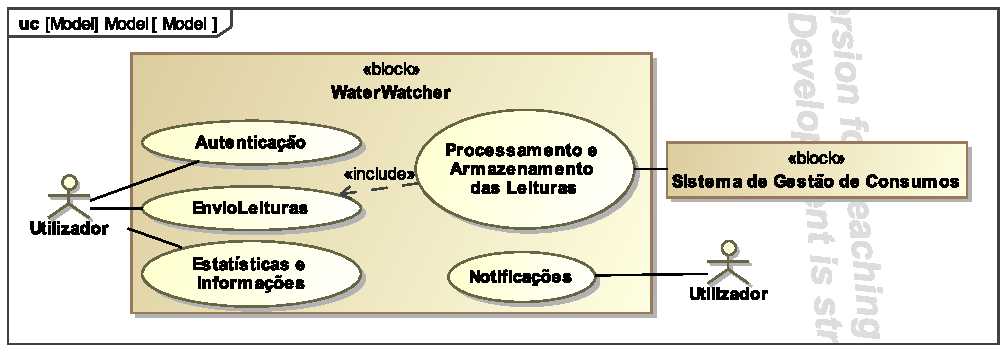
\includegraphics{diagramas/svg/uc__Model.pdf}}
\caption{Casos de uso do sistema.}
\label{fig:uso_sistema}
\end{center}
\end{figure}

O sistema, de forma geral, permitirá ao utilizador autenticar-se, submeter as leituras de água e aceder a informações relacionadas com o seu consumo. Após receber a leitura de água do utilizador, o sistema irá processar essa informação e posteriormente enviá-la para o sistema de gestão de consumos. Por fim, o sistema também poderá enviar notificações relativas ao serviço para o utilizador.\\
Analisámos também os casos de uso específicos para cada componente do sistema, analisando as funções de cada um e as suas interações tanto com utilizadores como com outros componentes do sistema ou até outros sistemas. A secção \label{sec:casos_servidor} descreve os casos de uso do servidor enquanto que a secção \label{sec:casos_iu} descreve os casso de uso da interface do utilizador.

% CASOS DE USO DO SERVIDOR
\section{Casos de Uso do Servidor} \label{sec:casos_servidor}
Na figura \ref{fig:uso_serv1} estão presentes os casos de utilização em que o ator, ou seja, onde se iniciam as ações que promovem os processos no sistema, é a interface de utilizador, enquanto que na figura \ref{fig:uso_serv2} o ator é a empresa fornecedora ou a interface de utilização.

\vspace{2cm} %espaço

\begin{figure}[h!]
\begin{center}
\resizebox{130mm}{!}{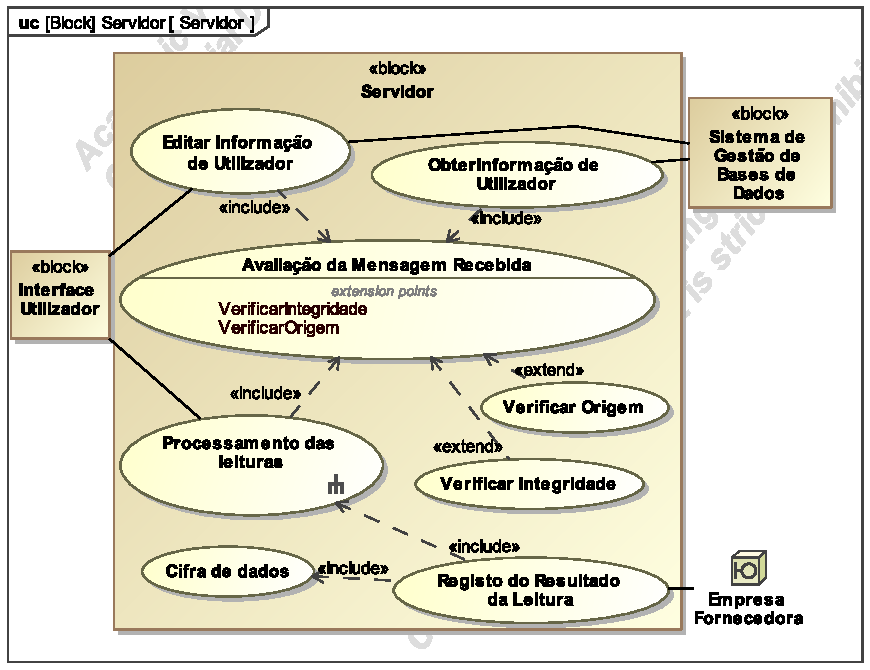
\includegraphics{diagramas/svg/uc__Servidor__Servidor.pdf}}
\caption{Casos de uso do servidor pela interface do utilizador.}
\label{fig:uso_serv1}
\end{center}
\end{figure}

O servidor está encarregado de receber as fotografias dos contadores enviadas pelos utilizadores e processá-las, ou seja, interpretar os caracteres na fotografia do contador para obter o resultado da contagem e enviar esse resultado para o sistema informático da empresa fornecedora de água.\\
Também é o responsável por mediar as interações das interfaces de utilização com a base de dados que contém a informação dos utilizadores, confirmando se o utilizador que fez o pedido pode ter acesso às informações que pede, efetuar o pedido à base de dados e enviar o resultado para o cliente que fez o pedido.\\
Qualquer mensagem recebida tem de ser avaliada para garantir a sua origem e garantir que o conteúdo não se alterou no processo da comunicação. As comunicações provenientes do servidor devem ser cifradas e assinadas de forma a que o destinatário saiba que foi, de facto, o servidor quem enviou essa mensagem e que o conteúdo da mensagem não sofreu alterações indevidas e também para que o conteúdo da mensagem não seja visível para alguém que tenha acesso indevido à mensagem durante o seu transporte.\\

\vspace{2.5cm} %espaço

\begin{figure}[h!]
\begin{center}
\resizebox{110mm}{!}{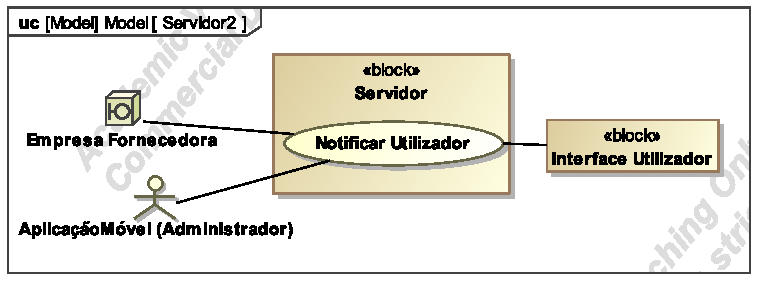
\includegraphics{diagramas/svg/uc__Servidor2.pdf}}
\caption{Casos de uso do servidor pela empresa fornecedora ou pelo administrador.}
\label{fig:uso_serv2}
\end{center}
\end{figure}

Quanto às interações promovidas pelos administradores ou pela empresa fornecedora, estas poderão submeter notificações para um ou vários utilizadores, pelo que o servidor depois encaminhará essas notificações para os utilizadores corretos.

A figura \ref{fig:state_processamento} representa o processamento das leituras pelo servidor.

\begin{figure}[h!]
\begin{center}
\resizebox{110mm}{!}{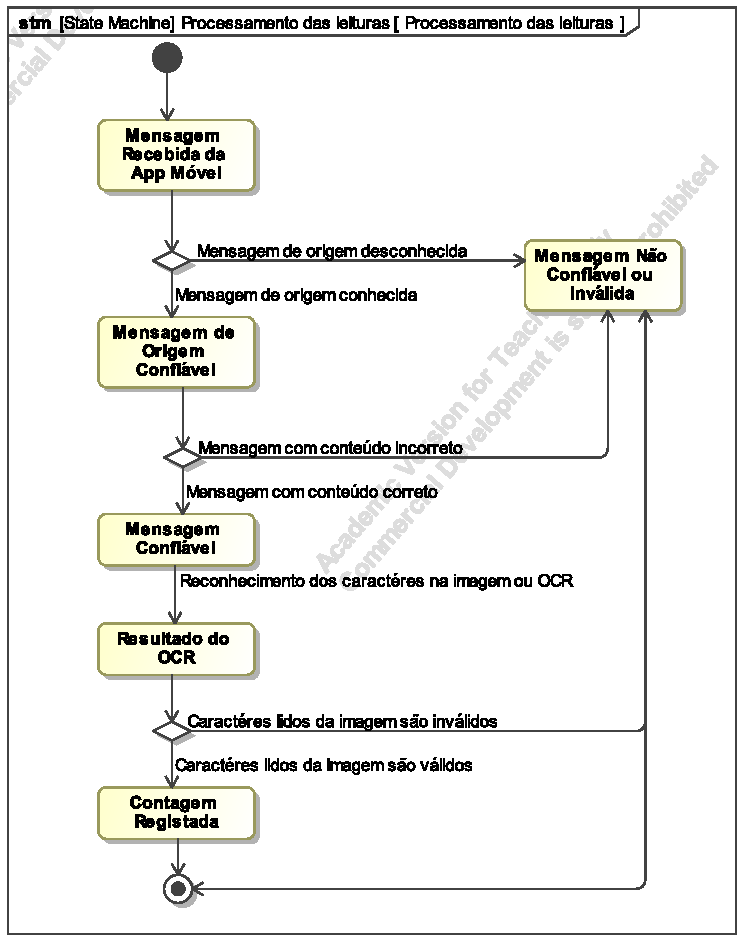
\includegraphics{diagramas/svg/stm__Processamento_das_leituras__Processamento_das_leituras.pdf}}
\caption{Processamento das leituras dos contadores.}
\label{fig:state_processamento}
\end{center}
\end{figure}

O processamento das leituras consiste inicialmente em verificar a origem e a integridade da mensagem recebida, descartando a mensagem caso o sistema detete que a mensagem não deva ser processada. Posteriormente é efetuado o reconhecimento dos caracteres na imagem e, caso o resultado deste processo apresente um valor válido para uma leitura, a contagem é registada para o utilizador que enviou a mensagem inicial.

% CASOS DE USO DA APP MOVEL
\section{Casos de Uso da Interface de Utilização} \label{sec:casos_iu}
A interface de utilização também tem vários casos de utilização, apresentados na figura \ref{fig:uso_iu}.

\begin{figure}[h!]
\begin{center}
\resizebox{140mm}{!}{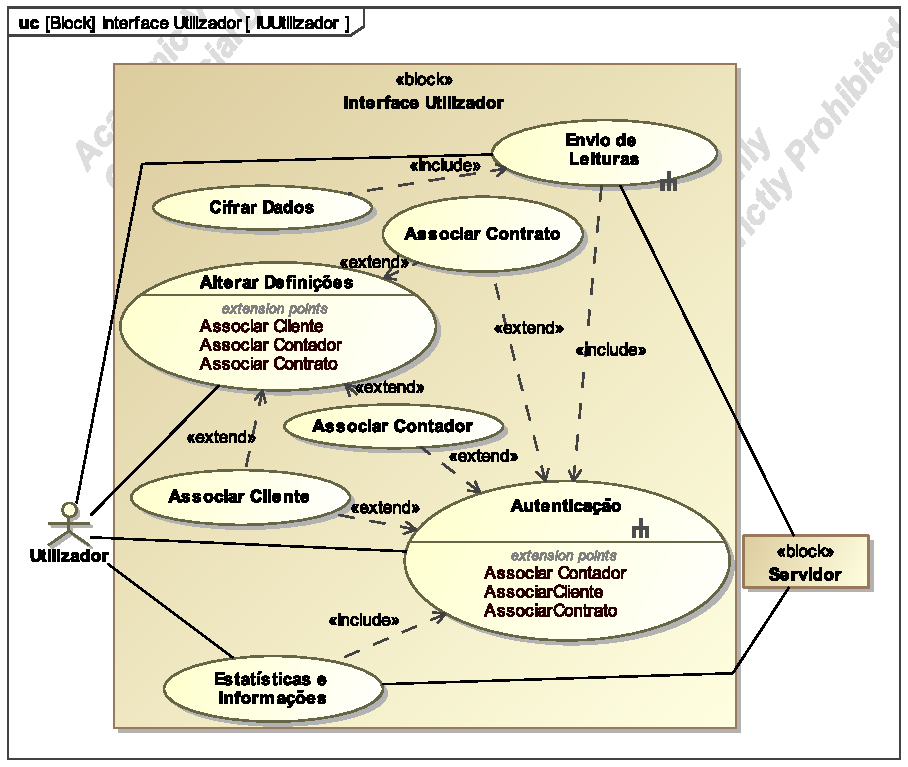
\includegraphics{diagramas/svg/uc__Interface_Utilizador__IUUtilizador.pdf}}
\caption{Casos de uso da interface de utilização.}
\label{fig:uso_iu}
\end{center}
\end{figure}

A interface de utilização é a parte do sistema que trata a interação com os utilizadores. É aqui que o utilizador se autentica, ou seja, efetua o seu registo quando utiliza o sistema pela primeira vez, sendo que nos próximos acessos será naturalmente apenas necessário o {\textit{log in}}.\\
Poderá posteriormente adicionar ou remover contadores e contratos, bem como alterar as suas informações pessoais. O utilizador pode ter acesso às suas estatísticas de consumo de água e a outras informações relativas ao serviço.\\
Também poderá então captar uma fotografia do contador para iniciar o processo de informar a empresa da sua contagem de água. À semelhança do servidor, as comunicações deverão ser cifradas e assinadas pelos mesmos motivos.\\

A autenticação, descrita na figura \ref{fig:state_autenticacao}, consiste em permitir ao utilizador criar uma conta nova ou aceder com as credenciais de uma conta já existente.

\begin{figure}[ht!]
\begin{center}
\resizebox{110mm}{!}{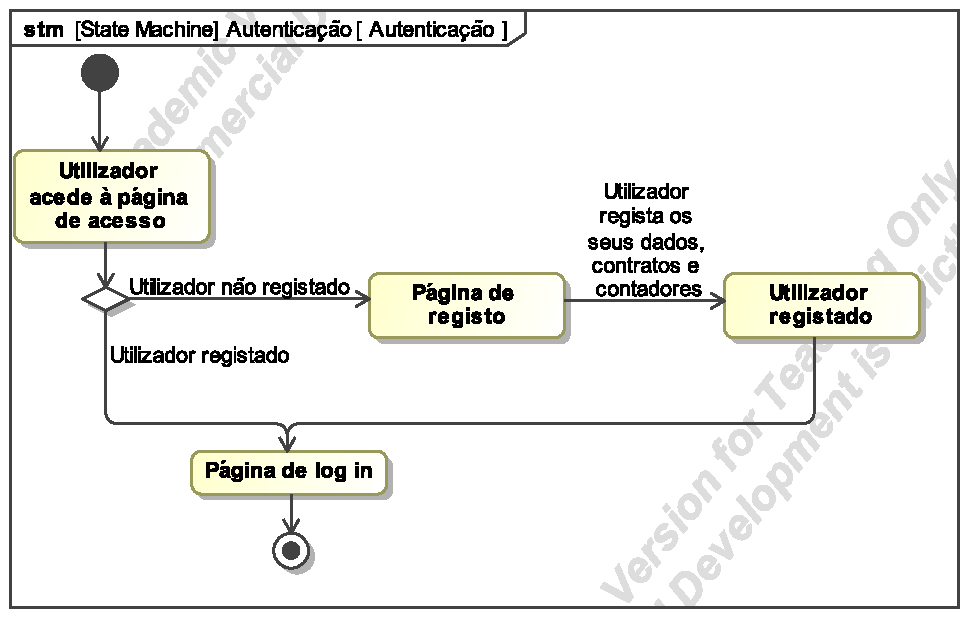
\includegraphics{diagramas/svg/stm__Autenticação__Autenticação.pdf}}
\caption{Processo de autenticação.}
\label{fig:state_autenticacao}
\end{center}
\end{figure}

A figura \ref{fig:state_envio} descreve o processo de envio de leituras.

\begin{figure}[ht!]
\begin{center}
\resizebox{95mm}{!}{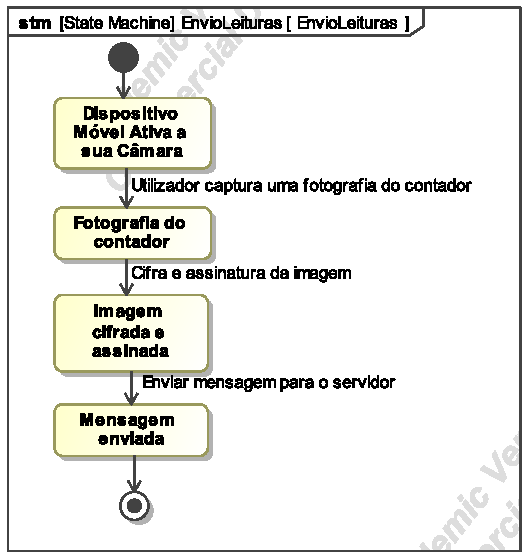
\includegraphics{diagramas/svg/stm__EnvioLeituras__EnvioLeituras.pdf}}
\caption{Processo de envio de leituras.}
\label{fig:state_envio}
\end{center}
\end{figure}

O processo de envio de leituras começa com a ativação da câmara do dispositivo do utilizador de forma a que este possa captar uma fotografia do seu contador. Depois de tirada a fotografia, este elemento gera uma mensagem que contém esta fotografia, cifra e assina esta mensagem e envia-a para o servidor.












% Capitulo 4
\chapter{Estratégias de Abordagem aos Problemas} \label{cap:abordagem}
Neste capítulo vamos analisar os procedimentos, tecnologias e conceitos utilizados no desenvolvimento deste projeto. Na secção \ref{sec:dados} propomos um modelo para a estrutura de dados utilizada neste sistema. Na secção \ref{sec:ecra} vamos apresentar esboços para os ecrãs da aplicação para os utilizadores.

%MODELO DE DADOS ......................................................................................
\section{Modelo de Dados} \label{sec:dados}
Um dos componentes deste sistema é um repositório de dados, que irá conter as várias informações relacionadas com os clientes deste serviço. Na figura \ref{fig:relacoes} está representado de forma gráfica o modelo dos dados guardados neste repositório. \\

\begin{figure}[ht!]
\centering
\resizebox{90mm}{!}{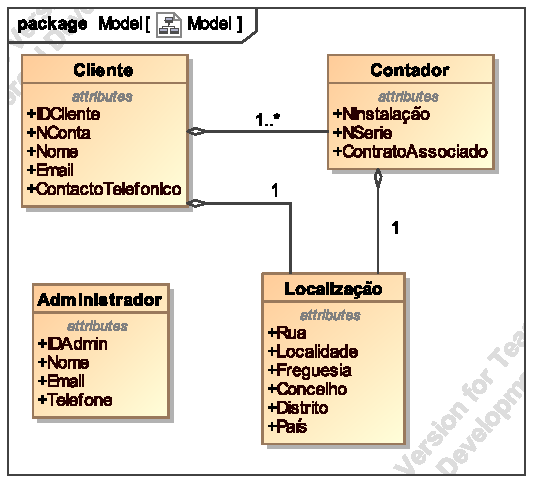
\includegraphics{diagramas/svg/uml__Model.pdf}}
\caption{Arquitetura do sistema.}
\label{fig:relacoes}
\end{figure}

O elemento cliente representa um cliente do serviço que utiliza o sistema. Para cada cliente será registado um ID único  \texttt{(IDCliente)}, o seu \texttt{nome}, \texttt{email}, número de telefone/telemóvel (\texttt{Telefone}) e \texttt{número de conta}. \\
Também existem utilizadores com papel de administrador, para os quais registamos um ID único (\texttt{IDAdmin}), o seu \texttt{nome}, \texttt{email} e número de telefone/telemóvel(\texttt{Telefone}) . \\
Os clientes terão associado um ou mais contadores, pelo que para cada contador guardamos o seu número único de instalação (\texttt{NInstalação}), o seu número de série (\texttt{NSerie}) e o contrato (\texttt{ContratoAssociado}) e o cliente (\texttt{IDCliente}) aos quais este contador está associado. \\
Cada contador tem uma localização, que representa o local onde o contador está instalado. Cada cliente tem também uma localização associada, que representa a sua morada principal para onde é, por exemplo, enviado o correio postal. Uma localização segue a estrutura normal de uma morada: \texttt{rua}, \texttt{localidade}, \texttt{freguesia}, \texttt{concelho}, \texttt{distrito} e \texttt{país}.

%ECRAS ...........................................................................................................
\section{Ecrãs da Aplicação Móvel} \label{sec:ecra}
Nesta secção apresentamos os vários esboços que desenhámos para os ecrãs ou páginas da aplicação móvel.\\
Na figura \ref{fig:1} está a página de \textit{log-in}.

\begin{figure}[ht!]
\centering
\resizebox{40mm}{!}{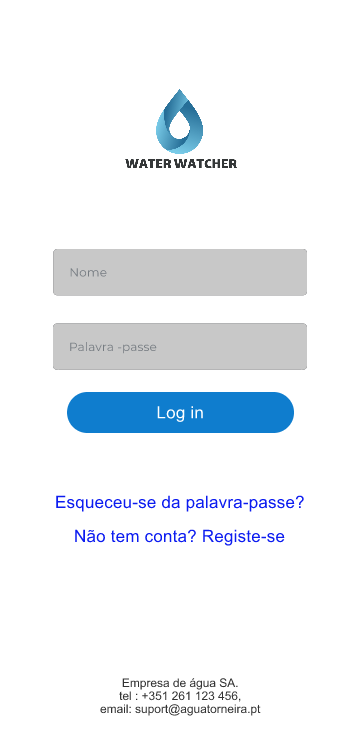
\includegraphics{diagramas/app/1.png}}
\caption{Página de log-in.}
\label{fig:1}
\end{figure}

Nesta página é possível o utilizador inserir as suas credenciais para entrar na aplicação. Também é possível registar uma nova conta ou recuperar o acesso a uma conta. Esta página apresenta também os contactos da empresa.\\
Depois de efetuado o \textit{log-in}, o utilizador é encaminhado para a página principal, apresentada na figura \ref{fig:2}.

\begin{figure}[ht!]
\centering
\resizebox{40mm}{!}{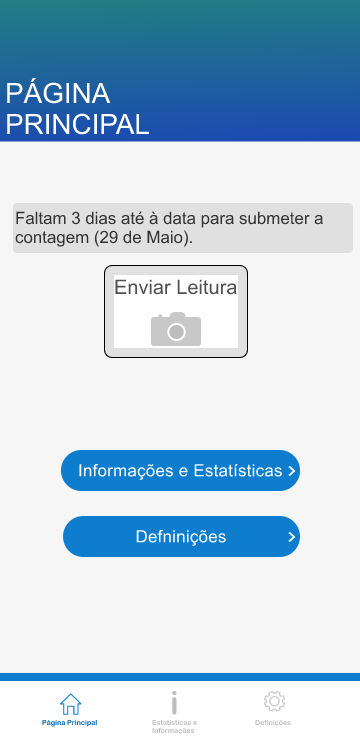
\includegraphics{diagramas/app/2.png}}
\caption{Página principal}
\label{fig:2}
\end{figure}

É neste ecrã que o utilizador poderá enviar a fotografia do contador no dia designado. \\
A partir deste ecrã, tem também a possibilidade de aceder às informações e estatísticas presentes no ecrã representado na figura \ref{fig:3}. 

%\vspace{8.5cm}

\begin{figure}[ht!]
\centering
\resizebox{40mm}{!}{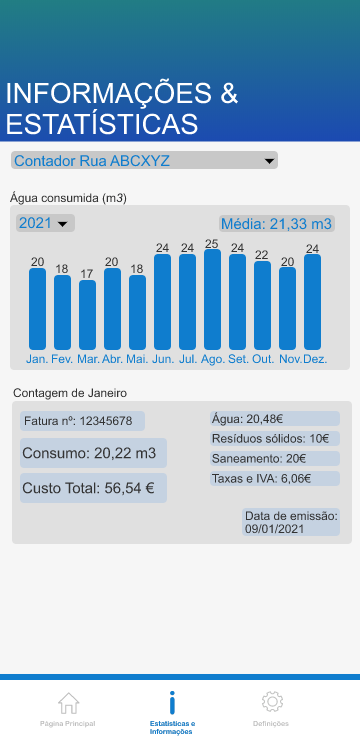
\includegraphics{diagramas/app/3.png}}
\caption{Página de informações e estatísticas}
\label{fig:3}
\end{figure}

A página de informações e estatísticas é onde estão disponíveis vários dados referentes ao serviço e detalhes das faturas do utilizador.\\ 
Por fim, é possível aceder ao ecrã de definições representado na figura \ref{fig:4}.

\vspace{1cm}

\begin{figure}
\centering
\begin{minipage}{.5\textwidth}
 \centering
\resizebox{40mm}{!}{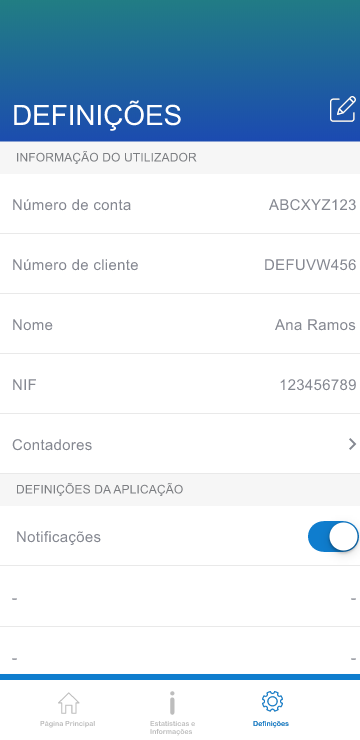
\includegraphics{diagramas/app/4.png}}
\caption{Página de definições.}
\label{fig:4}
\end{minipage}%
\begin{minipage}{.5\textwidth}
  \centering
\resizebox{40mm}{!}{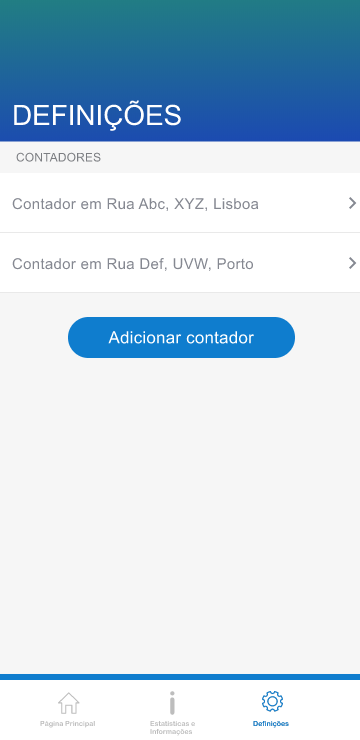
\includegraphics{diagramas/app/5.png}}
\caption{Página de definições relacionadas com os contadores.}
\label{fig:5}
\end{minipage}
\end{figure}

Nesta página, o utilizador pode ver e editar as suas informações e preferências da aplicação. Mais concretamente, também é possível gerir os contadores associados à sua conta, no ecrã da figura \ref{fig:5}.

\section{Reconhecimento de Caracteres} \label{caracteres}
Este sistema vai reconhecer caracteres presentes nas fotografias dos contadores dos clientes. Para melhorar a qualidade e eficácia do reconhecimento de caracteres decidimos estudar e testar vários tipos de imagens de um contador para perceber em quais é que o reconhecimento de caracteres era mais eficaz.
Para este teste utilizamos as seguintes imagens:\\
\par1-Imagem digital de números pretos em fundo branco, de referência.
\par2-Fotografia do contador.
\par3-Fotografia do contador cortada de forma a só conter o mostrador dos números.
\par4-Fotografia 3 em preto e branco.
\par5-Fotografia 3 com as cores invertidas.
\par6-Fotografia 3 com as dimensões aumentadas.\\

Obtivemos mais sucesso, ou seja, o texto obtido através do reconhecimento de caracteres ser mais próximo dos números reais presentes no contador, com a fotografia restringida ao mostrador do contador com as cores invertidas.

\section{Programa de Controlo Semanal} \label{rec}
Existirá uma forma de os clientes do serviço poderem ter um maior controlo do seu consumo de água, nomeadamente, saber o seu gasto em períodos menores do que mensalmente.\\
Propomos a implementação de um processo, totalmente opcional e que não interfere com a restante utilização do sistema, que lembra os utilizadores semanalmente de enviar a contagem do seu contador.\\
Estes envios terão como propósito poder apresentar ao utilizador o seu gasto de água semanal, permitindo que este, por exemplo, alterando os seus hábitos de consumo de água, consiga observar alterações mais imediatas nas suas contagens. Por outro lado, a empresa terá também acesso a estas contagens.\\
Estas contagens têm uma função meramente informativa e são de carater opcional.


\section{Biblioteca de Reconhecimento de Caracteres} \label{rec}
Para o reconhecimento de caracteres elaborámos uma extensão Outsystems que tem por base a biblioteca Tesseract \cite{tesseract}.\\
A biblioteca Tesseract é uma biblioteca open source muito utilizada no reconhecimento de caracteres em imagem por ser facilmente configurável consoante a linguagem ou tipo de caracteres que se pretende extrair. Implementa uma rede neuronal para a deteção dos caracteres e utiliza um ficheiro de configuração configurado para detetar dígitos presente em \ref{tes:digits}.




















% Capitulo 5
\chapter{Aspetos da Implementação} \label{cap:implementacao}
Esta secção tem como propósito clarificar e justificar as várias decisões que tomámos no desenvolvimento dos vários módulos do projeto. \\
Na secção \ref{sec:ecra} iremos apresentar os vários ecrãs da aplicação móvel desenvolvida.

\section{Ecrãs da aplicação móvel} \label{sec:ecra}
Nesta secção apresentamos os vários ecrãs ou páginas da aplicação móvel. Na figura \ref{fig:1} está a página de \textit{log-in}, onde é possível o utilizador inserir o seu [nome, username] e a sua palavra-passe. Também é possível registar uma nova conta ou recuperar o acesso à conta do utilizador. Esta página apresenta também os contactos da empresa.\\
Depois de efetuado o \textit{log-in}, o utilizador é encaminhado para a página principal, apresentada na figura \ref{fig:2}, onde poderá enviar a fotografia do contador no dia designado. \\
Terá também a possibilidade de aceder à página de informações e estatísticas representada na figura \ref{fig:3}, onde estão disponíveis vários dados referentes ao serviço e detalhes das faturas do utilizador.\\ Por fim, é possível aceder ao ecrã \ref{fig:4}, onde o utilizador pode ver e editar as suas informações e preferências da aplicação. Mais concretamente, também é possível gerir os contadores associados á sua conta, no ecrã da figura \ref{fig:5}.

\begin{figure}
\centering
\begin{minipage}{.5\textwidth}
\centering
\resizebox{50mm}{!}{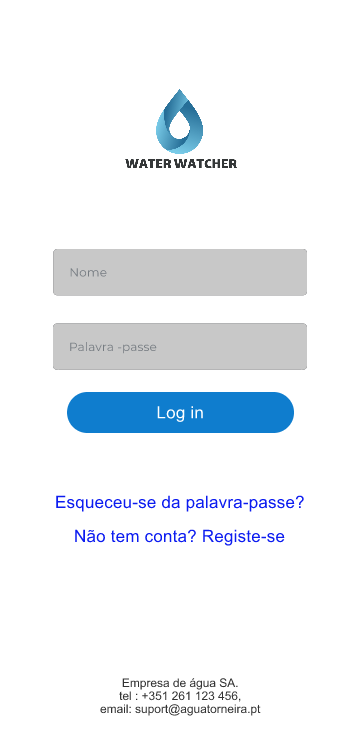
\includegraphics{diagramas/app/1.png}}
\caption{Página de log-in.}
\label{fig:1}
\end{minipage}%
\begin{minipage}{.5\textwidth}
\centering
\resizebox{50mm}{!}{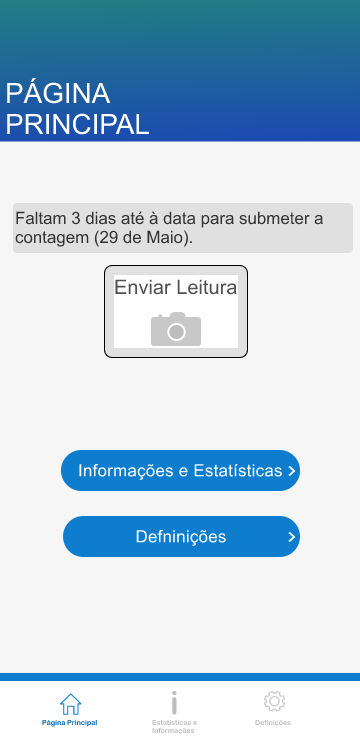
\includegraphics{diagramas/app/2.png}}
\caption{Página principal}
\label{fig:2}
\end{minipage}
\end{figure}

\begin{figure}
\centering
\begin{minipage}{.5\textwidth}
\centering
\resizebox{50mm}{!}{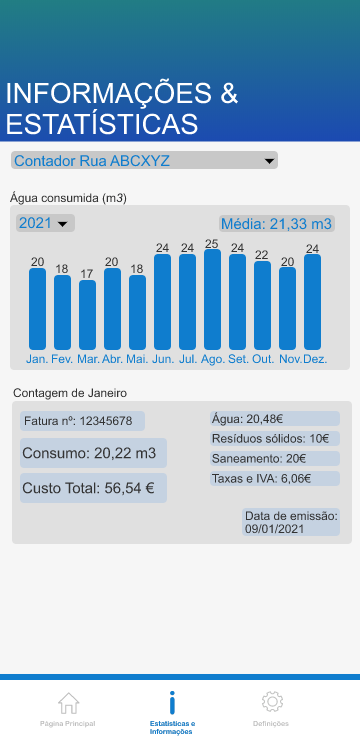
\includegraphics{diagramas/app/3.png}}
\caption{Página de informações e estatísticas}
\label{fig:3}
\end{minipage}%
\begin{minipage}{.5\textwidth}
\centering
\resizebox{50mm}{!}{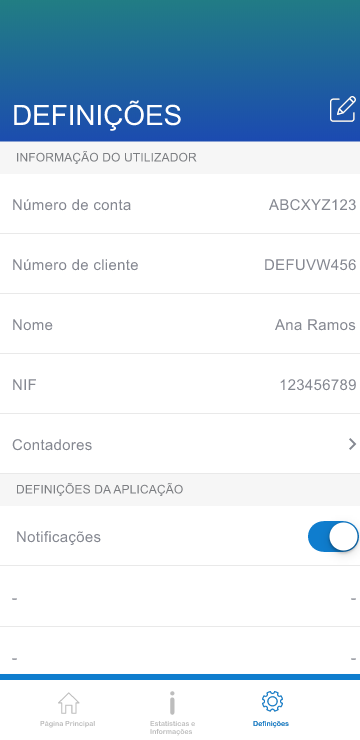
\includegraphics{diagramas/app/4.png}}
\caption{Página de definições.}
\label{fig:4}
\end{minipage}
\end{figure}

\begin{figure}[ht!]
\centering
\resizebox{50mm}{!}{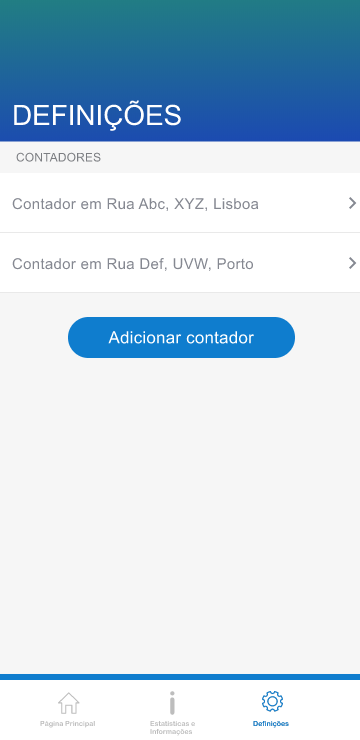
\includegraphics{diagramas/app/5.png}}
\caption{Página de definições relacionadas com os contadores.}
\label{fig:5}
\end{figure}




% Capitulo 6
%\chapter{Testes} \label{cap:testes}

Este é o capítulo de testes. 
É possível forçar a inclusão de todas as referências com \cite{*}.

Modo de matemática em texto $x = ma^2$ e em equação (duas formas):
\[
    x = ma^2
\]

\begin{equation}
    x = ma^2
\end{equation}


% Referências
\nocite{*}
\bibliographystyle{unsrt}
\bibliography{referencias}
\addcontentsline{toc}{chapter}{Refer\^{e}ncias}

% Apêndices (opcional)
%\newacronym{smas}{SMAS}{Serviços Municipalizados de Água e Saneamento}
\newacronym{pwa}{PWA}{Progressive Web Applications}
\newglossaryentry{interface}
{
    name=interface,
    description={Apresentação gráfica dos dados e funcionalidades de um elemento.}
}

%
% Apêndice 1
%
\chapter{Exemplo de apêndice} \label{ap:exemplo}
Este é o primeiro parágrafo do apêndice.


\lipsum[14-16]

\end{document} 